\documentclass[12pt]{article}

% --- Core Math Packages ---
\usepackage{amsmath}
\usepackage{amssymb} % Provides \mathbb, \mathfrak, etc.
\usepackage{amsfonts} % Provides math fonts
\usepackage{amsthm}   % Theorem environments
\usepackage{mathtools} % Extends amsmath, e.g., \coloneqq
\usepackage{mathrsfs}  % Provides \mathscr
\usepackage{tikz-cd} % For commutative diagrams

% --- Page Layout & Typography ---
\usepackage{geometry} % For margin control
\usepackage{lmodern} % Use Latin Modern fonts (pairs well with T1)
\usepackage[T1]{fontenc} % Font encoding (improves copy-paste, hyphenation)
\usepackage[utf8]{inputenc} % Input encoding (allows UTF-8 characters)
\usepackage{microtype} % Improved typography (subtle adjustments)
\usepackage[english]{babel} % Uncomment if writing primarily in English for hyphenation etc.

% --- Graphics, Links, Lists, Tables ---
\usepackage{graphicx} % For including images
\usepackage{hyperref} % For clickable links (references, URLs)
\usepackage{tikz}     % For drawing diagrams (if needed later)
\usepackage{enumitem} % For customizing lists (like C1, C2...)
\usepackage{booktabs} % For professional-looking tables (if needed later)
\usepackage{url}      % For typesetting URLs

% --- Page Geometry ---
\geometry{margin=1in} % Set 1-inch margins on all sides

% --- Theorem Environments ---
% Numbered within sections
\newtheorem{definition}{Definition}[section]
\newtheorem{lemma}{Lemma}[section]
\newtheorem{proposition}{Proposition}[section]
\newtheorem{corollary}{Corollary}[section]
\newtheorem{theorem}{Theorem}[section]

% --- Custom Math Commands (Examples from original doc) ---
% Add your specific commands here as needed, e.g.:
% \DeclareMathOperator{\arcsinh}{arcsinh}

% --- Document Metadata ---
\title{Arithmetic Expression Geometry I: Flow, Torsion, and the First Kind Expression Space}
\author{Mingli Yuan \\ % Affiliation can be added here if desired
        \texttt{mingli.yuan@gmail.com}} % Example email
\date{\today} % Use current date for drafts

% --- Hyperref Setup (Optional Customization) ---
\hypersetup{
    colorlinks=true,
    linkcolor=blue,
    filecolor=magenta,
    urlcolor=cyan,
    citecolor=green,
    pdftitle={\@title}, % Use title for PDF metadata
    pdfauthor={\@author}, % Use author for PDF metadata
    pdfkeywords={Arithmetic Expressions, Hyperbolic Geometry, Flow Equation, Geometric Group Theory, Computational Geometry, Arithmetic Torsion}, % Add keywords
    bookmarks=true,
    bookmarksopen=true,
}

% --- Document Start ---
\begin{document}

\maketitle

\begin{abstract}
We introduce a novel geometric framework, \emph{Arithmetic Expression Geometry} (AEG), which interprets arithmetic expressions as propagating structures embedded in curved geometric spaces. This paper constructs the foundational model---the \emph{first kind expression space} \( \mathfrak{E}_1 \)---on the upper half-plane with a hyperbolic metric structure. We derive a flow equation governing the propagation of values along arithmetic paths and show that the assignment function \( a = -x/y \) satisfies this flow equation. For the standard Poincaré metric case (\(\mu=1, \lambda=1\)), \(a\) is also an eigenfunction of the Laplacian with eigenvalue -2. We establish a precise correspondence between local arithmetic torsion, which captures the non-commutativity of addition and multiplication, and hyperbolic area in grid structures embedded in \( \mathfrak{E}_1 \). Furthermore, we define a global arithmetic torsion for arbitrary expression paths and prove a triple identity relating it to a geometric area integral within a specially constructed 'accumulative commutative space', providing a Stokes-like theorem for arithmetic. Finally, we introduce the tube structure \( \mathcal{T} \) to study parameterized expression families. This work establishes the theoretical foundation for a geometry of computation rooted in arithmetic structure.
\end{abstract}

\tableofcontents
\newpage

\section{Introduction}

\subsection{Historical Context and Motivation}
The study of arithmetic expressions has deep roots, extending from foundational work on formal grammars and rewriting systems (e.g., Post\cite{Post1943FormalRO}, Chomsky\cite{Chomsky1956ThreeMF}) to the development of type theory and lambda calculus aimed at taming paradoxes and managing computational semantics (e.g., Church\cite{Church1940AFO}, Martin-L\"{o}f\cite{MartinLf1975AnIT}). These traditions primarily treat expressions as symbolic or algebraic objects—trees, terms, strings—subject to syntactic rules and evaluation procedures. While powerful, this perspective often overlooks potential intrinsic geometric structures. This leads to a fundamental question, largely unexplored: \textit{Can the very process of arithmetic evaluation manifest as a geometric phenomenon?} Can expressions trace paths, define flows, and inhabit spaces shaped by the operations themselves?

\subsection{Main Research Question}
This paper addresses the central theoretical question:
\begin{center}
\emph{Can the dynamics of evaluating arithmetic expressions be intrinsically encoded in a geometric space, with propagation governed by inherent rules?}
\end{center}
We propose such a geometry exists, where fundamental operations like addition and multiplication correspond to motions along distinct directions within a curved space, and the evaluation process unfolds dynamically as a geometric flow. In this view, arithmetic operations generate not just numbers, but geometric structures: they induce \emph{flows}, accumulate \emph{torsion}, and define \emph{paths} through dedicated mathematical spaces.

\subsection{Core Contributions}
This paper, the first in a planned series, establishes the foundations of Arithmetic Expression Geometry by presenting its major contributions:
\begin{enumerate}[label=\textbf{C\arabic*.}, leftmargin=*, widest=C5, align=left]
  \item We define \textbf{threadlike arithmetic expressions} and formalize their representation via curried path notation, providing a tractable model for sequential computation.
  \item We derive the \textbf{arithmetic flow equation} that governs how expression values propagate along these paths and demonstrate its interpretation as a special Eikonal equation from geometric optics and mechanics.
  \item We construct the \textbf{first kind arithmetic expression space} \( \mathfrak{E}_1 \) on the upper half-plane equipped with a general hyperbolic metric structure, where the assignment function \( a = -x/y \) satisfies the flow equation and is a Laplacian eigenfunction.
  \item We introduce \textbf{arithmetic torsion}, quantifying the non-commutativity of addition and multiplication, and establish both a local correspondence to hyperbolic area in \( \mathfrak{E}_1 \) and a global integral identity in a separate 'accumulative commutative space'.
  \item We propose the \textbf{tube structure} \( \mathcal{T} \), formed by parameterizing families of expression spaces, providing a framework to study the dynamics of expressions and the evolution of their zero loci across parameters.
\end{enumerate}

\subsection{Organization of the Paper}
The remainder of this paper is structured as follows:
\begin{itemize}
  \item \textbf{Section 2} formally defines arithmetic expressions as paths using production rules, currying, and path notation, focusing on threadlike and alternating structures.
  \item \textbf{Section 3} derives the arithmetic flow equation from infinitesimal generation principles and analyzes its Eikonal, Hamilton-Jacobi, and contour-gradient forms.
  \item \textbf{Section 4} constructs the first kind space \( \mathfrak{E}_1 \), establishes its metric structure, and proves the properties of the assignment function \(a=-x/y\).
  \item \textbf{Section 5} investigates geometric phenomena within \( \mathfrak{E}_1 \), including expression propagation mechanisms, dual grid structures related to Baumslag–Solitar groups, and the local torsion-area correspondence.
  \item \textbf{Section 6} introduces global arithmetic torsion, the accumulative commutative space, and establishes an integral theorem for torsion.
  \item \textbf{Section 7} introduces the tube structure \( \mathcal{T} \) as a family of \( \mathfrak{E}_1 \) spaces, discussing sections, trajectories, and the potential for complex zero locus evolution.
  \item \textbf{Section 8} provides a discussion of the results and outlines future research directions, including curvature interpretations, integral theorems, and connections to other mathematical fields.
\end{itemize}

\section{Threadlike Expressions and Arithmetic Paths}\label{sec:paths_cs}

This section lays the algebraic groundwork for Arithmetic Expression Geometry (AEG). We formally define arithmetic expressions, focusing on a computationally significant subclass known as threadlike expressions. We then introduce path notation via currying, establishing a framework where sequences of arithmetic operations are treated as composable paths, analogous to structures studied in formal language theory and geometric group theory.

\subsection{Syntactic Structure and Evaluation}

We begin by defining the fundamental objects of our study: arithmetic expressions built over the field of rational numbers \( \mathbb{Q} \). While our ultimate goal involves geometric spaces potentially related to real or complex numbers, starting with \( \mathbb{Q} \) avoids immediate complications related to decidability and singularities (issues discussed further in Section~\ref{sec:discussion_future}).

\begin{definition}[Arithmetic Expression]\label{def:arithmetic_expression_cs}
An \textbf{arithmetic expression} \( a \) over the rational numbers \( \mathbb{Q} \) is a structure inductively defined by the following grammar:
\begin{equation*}
a \longleftarrow x \quad | \quad (a + a) \quad | \quad (a - a) \quad | \quad (a \times a) \quad | \quad (a \div a),
\end{equation*}
where \( x \in \mathbb{Q} \). The set of all such expressions is denoted by \( \mathbb{E}[\mathbb{Q}] \).
\end{definition}

Each expression \( a \in \mathbb{E}[\mathbb{Q}] \) admits both a familiar string representation (e.g., \( ((1+2)\times 3) \)) and an equivalent, unique tree representation where internal nodes are operators (\(+, -, \times, \div\)) and leaf nodes are rational constants (\(x \in \mathbb{Q}\)).

The semantics are given by a partial evaluation function \( \nu: \mathbb{E}[\mathbb{Q}] \dashrightarrow \mathbb{Q} \), defined recursively in the standard way:
\begin{itemize}
    \item \( \nu(x) = x \) for any \( x \in \mathbb{Q} \).
    \item \( \nu((a \mathbin{op} b)) = \nu(a) \mathbin{op} \nu(b) \) for \( \mathrm{op} \in \{+, -, \times\} \), provided \( \nu(a) \) and \( \nu(b) \) are defined.
    \item \( \nu((a \div b)) = \nu(a) / \nu(b) \), provided \( \nu(a) \), \( \nu(b) \) are defined and \( \nu(b) \neq 0 \).
\end{itemize}
An expression \( a \) is \textbf{evaluable} if \( \nu(a) \) is defined. Unless otherwise stated, we will primarily consider evaluable expressions in this foundational work.

\subsection{Threadlike Expressions and Currying}

While general arithmetic expressions correspond to arbitrary trees, we focus on a specific class that reflects sequential computation.

\begin{definition}[Threadlike Expression]\label{def:threadlike_expression_cs}
A \textbf{threadlike expression} is an arithmetic expression whose syntax tree has the property that every left child of any internal node is a leaf node (a constant).
\end{definition}

Threadlike expressions correspond to fully right-associated or right-nested structures. A key property of threadlike expressions is that they possess a \textbf{unique evaluation order}, proceeding strictly from the innermost operation outwards. This sequential structure lends itself naturally to representation using \emph{currying}, transforming the expression into a sequence of unary function applications acting on an initial operand. To align with the geometric interpretation developed later, we define the core path operators as follows:

\begin{definition}[Path Operators]\label{def:path_operators_cs}
Let \( \mu, \lambda \in \mathbb{R} \).
\begin{itemize}
  \item Additive operator: \( \oplus_\mu : x \mapsto x + \mu \)
  \item Subtractive operator: \( \ominus_\mu : x \mapsto x - \mu \)
  \item Multiplicative operator: \( \otimes_\lambda : x \mapsto x \cdot e^\lambda \)
  \item Divisive operator: \( \oslash_\lambda : x \mapsto x \cdot e^{-\lambda} \)
\end{itemize}
\end{definition}
The use of \( e^\lambda \) is crucial for the connection to hyperbolic geometry and the flow equation derived in Section~\ref{sec:flow_equation_cs}.

\begin{definition}[Path Notation]\label{def:path_notation_cs}
Let \( x \in \mathbb{Q} \) be an initial operand and \( a_1, a_2, \dots, a_n \) be a sequence of path operators. The \textbf{path notation} represents the sequential application:
\[
x a_1 a_2 \dots a_n \coloneqq a_n(\cdots a_2(a_1(x)) \cdots)
\]
A path starting with an initial operand \( x \) is a \textbf{bounded path}. A sequence of operators without an initial operand is a \textbf{free path}, representing a function.
\end{definition}

\subsection{Associativity and Concatenation of Paths}

Paths can be combined through concatenation, which corresponds to function composition.

\begin{definition}[Path Concatenation]\label{def:concatenate_cs}
The \textbf{concatenation} of two free paths \( p_1 \) and \( p_2 \) is \( p_1 \cdot p_2 \). The corresponding function is \( \mathbf{p}_2 \circ \mathbf{p}_1 \).
\end{definition}

\begin{lemma}[Associativity of Path Application]\label{lemma:associative_cs}
The application of path operators is associative, inherited from the associativity of function composition.
\end{lemma}
\begin{proof}
Let \( \mathbf{a}, \mathbf{b}, \mathbf{c} \) be the functions for free paths \( a, b, c \). The path \( (a \cdot b) \cdot c \) corresponds to the function \( \mathbf{c} \circ (\mathbf{b} \circ \mathbf{a}) \). The path \( a \cdot (b \cdot c) \) corresponds to \( (\mathbf{c} \circ \mathbf{b}) \circ \mathbf{a} \). By associativity of function composition, these are identical.
\end{proof}

\subsection{Alternating Threadlike Expressions and Perturbation}

A particularly important subclass consists of paths where additive and multiplicative operations alternate.

\begin{definition}[Alternating Path]\label{def:alternating_path_cs}
An \textbf{alternating path} \( \alpha \) is a free path of the form:
\begin{equation}\label{eq:alternative_cs}
    \alpha = a_1 b_1 a_2 b_2 \cdots a_l b_l, \quad \text{where } a_i = \otimes_{\lambda_i}, \ b_i = \oplus_{\mu_i}
\end{equation}
\end{definition}

When applied to an initial value \( \mu_0 \), the result \( \alpha(\mu_0) \) can be expanded. Let \( \hat{\lambda}_k = \sum_{j=l-k+1}^{l} \lambda_j \) be the right-accumulated sum of multiplicative parameters. The evaluation expands to:
\begin{equation}
\alpha(\mu_0) = e^{\hat{\lambda}_l} \mu_0 + \sum_{i=1}^l e^{\hat{\lambda}_{l-i}} \mu_i \label{eq:alternating_expansion_cs}
\end{equation}
A perturbation at the start, \( \tilde{\mu}_0 \), propagates linearly:
\begin{equation}
\frac{\alpha(\tilde{\mu}_0) - \alpha(\mu_0)}{\tilde{\mu}_0 - \mu_0} = e^{\hat{\lambda}_l} = e^{\sum_{k=1}^l \lambda_k} \label{eq:ratio_cs}
\end{equation}
This shows that the sensitivity of the output to changes in the input depends only on the accumulated multiplicative factors.

\section{The Arithmetic Flow Equation}\label{sec:flow_equation_cs}

We now derive the central differential equation governing the continuous evolution of expression values within a geometric framework. This "Arithmetic Flow Equation" bridges discrete algebraic operations and continuous geometric propagation.

\subsection{Derivation from Infinitesimal Generation}

Consider a smooth assignment function \( a: M \to \mathbb{R} \) on a Riemannian manifold \( (M, g) \). We model its local generation via two orthogonal actions: an additive action with infinitesimal strength \( \mu \) and a multiplicative action with infinitesimal strength \( \lambda \). Moving an infinitesimal distance \( ds \) in a direction at angle \( \theta \) to the additive direction, the first-order change \( da \) is approximated by applying the actions in either order.
\begin{itemize}
    \item Add then multiply: \( (a + \mu ds \cos \theta) e^{\lambda ds \sin \theta} \approx a + a \lambda ds \sin \theta + \mu ds \cos \theta \)
    \item Multiply then add: \( a e^{\lambda ds \sin \theta} + \mu ds \cos \theta \approx a + a \lambda ds \sin \theta + \mu ds \cos \theta \)
\end{itemize}
Both yield the same first-order change. Taking the limit gives the directional derivative:
\begin{equation}
    \frac{da}{ds} = \mu \cos \theta + a \lambda \sin \theta \label{eq:flow_cs}
\end{equation}
This is the \textbf{Arithmetic Flow Equation}. It dictates how the value \( a \) changes as one moves on the manifold. A formal solution for constant \( \theta \) is derived in Appendix~\ref{app:flow_solution}.

\subsection{Eikonal and Hamilton–Jacobi Interpretation}

The flow equation can be expressed in a coordinate-free form. The maximum rate of change of \( a \), given by the norm of its gradient \( ||\nabla a|| \), must equal the maximum value of the right-hand side of Eq.~\eqref{eq:flow_cs} over all \( \theta \), which is \( \sqrt{\mu^2 + a^2 \lambda^2} \). This gives:
\begin{equation}\label{eq:coordinate_free_cs}
||\nabla a|| = \sqrt{\mu^2 + a^2 \lambda^2}
\end{equation}
This is an \textbf{Eikonal equation}, common in geometric optics. It is also equivalent to a static \textbf{Hamilton–Jacobi equation} \( H(x, a, \nabla a) = 0 \) with Hamiltonian:
\begin{equation}\label{eq:hamiltonian_cs}
    H(x, a, p) = ||p||_g - \sqrt{\mu^2 + a^2 \lambda^2}
\end{equation}
This connects AEG to the powerful frameworks of analytical mechanics.

\subsection{Contour-Gradient Coordinates and Propagation Laws}

We can analyze the flow in a local coordinate system based on the function \( a \) itself.
\begin{itemize}
    \item \textbf{Contour Direction:} Where \( da/ds = 0 \), we have \( \tan \theta_c = - \mu / (a \lambda) \).
    \item \textbf{Gradient Direction:} Orthogonal to the contour, the rate of change is maximal: \( \frac{da}{ds}\big|_{\theta_g} = \pm \sqrt{\mu^2 + a^2 \lambda^2} \).
\end{itemize}
Let \( \phi \) be the angle relative to the gradient direction. The flow equation becomes:
\begin{equation}
    \frac{da}{ds} = \sqrt {\mu^2 + a^2 \lambda^2} \cos \phi \label{eq:contourgradient_cs}
\end{equation}
Integrating this equation for a fixed direction \( \phi \) and initial condition \( a(0)=a_0 \) yields the explicit propagation law:
\begin{equation}
    a(s) = \frac{\mu}{\lambda} \sinh\left(\lambda s \cos \phi + \mathrm{arsinh} \frac{a_0 \lambda}{\mu}\right) \label{eq:gradevo_initial_cs}
\end{equation}
This solution describes how the value \( a \) evolves along straight lines in the local contour-gradient frame.

\section{The First Kind Expression Space \( \mathfrak{E}_1 \)}\label{sec:E1_space_cs}

We now construct the first concrete geometric realization of this framework: the \emph{first kind arithmetic expression space}, \( \mathfrak{E}_1 \), based on the upper half-plane model of hyperbolic geometry.

\subsection{Definition and Metric Structure}

The geometric foundation for \( \mathfrak{E}_1 \) is the upper half-plane manifold \( \mathcal{B} = \{ (x, y) \in \mathbb{R}^2 \mid y > 0 \} \). We equip it with a Riemannian metric \( g \) parameterized by \( \mu \) and \( \lambda \). The line element is:
\begin{equation}
ds^2 = \frac{1}{y^2}\left(\frac{dx^2}{\mu^2} + \frac{dy^2}{\lambda^2}\right) \label{eq:metric_general_cs}
\end{equation}
Within this space, we define the \textbf{assignment function} \( a: \mathcal{B} \to \mathbb{R} \) as:
\begin{equation}\label{eq:genassignment_cs}
a(x, y) = - \frac{x}{y}
\end{equation}

\begin{definition}[First Kind Expression Space]\label{def:E1_space_cs}
The \textbf{first kind arithmetic expression space} \( \mathfrak{E}_1(\mu, \lambda) \) is the Riemannian manifold \( (\mathcal{B}, g) \), with metric \( g \) from Eq.~\eqref{eq:metric_general_cs} and the distinguished assignment function \( a(x,y) = -x/y \).
\end{definition}

\subsection{Flow Equation and Laplacian Properties}

A key property is that this specific assignment function on this specific space satisfies our general flow equation.

\begin{theorem}[Assignment Satisfies Flow Equation]\label{thm:generalE1_cs}
In the space \( \mathfrak{E}_1(\mu, \lambda) \), the assignment function \( a(x,y) = -x/y \) satisfies the Arithmetic Flow Equation~\eqref{eq:flow_cs}.
\end{theorem}
\begin{proof}
The proof involves computing the differential \( da \), the arc length \( ds \), and forming the derivative \( da/ds \). By defining the angle \( \theta \) appropriately in terms of the scaled differentials \( dx/\mu \) and \( dy/\lambda \), the expression for \( da/ds \) simplifies to exactly \( \mu \cos \theta + a \lambda \sin \theta \). (See Appendix~\ref{app:geometry_calc} for details).
\end{proof}

The assignment function also has a special relationship with the Laplace-Beltrami operator \( \Delta_g \).

\begin{proposition}[Laplacian of the Assignment Function]\label{prop:laplacian_general_cs}
For the general \( \mathfrak{E}_1(\mu, \lambda) \) space, the assignment function \( a = -x/y \) is an eigenfunction of the Laplace-Beltrami operator \( \Delta_g = -\mathrm{div}(\mathrm{grad} f) \):
\[
\Delta_g a = -2\lambda^2 a
\]
\end{proposition}
\begin{proof}
The proof follows from a direct calculation using the coordinate formula for the Laplacian with the metric \( g \) from Eq.~\eqref{eq:metric_general_cs}.
\end{proof}

\begin{corollary}[Standard Poincaré Case]\label{cor:laplacian_standard_cs}
When \( \mu = 1 \) and \( \lambda = 1 \), the metric reduces to the standard Poincaré metric \( ds^2 = (dx^2 + dy^2)/y^2 \). In this standard hyperbolic space \( \mathfrak{E}_1(1, 1) \), the assignment function \( a = -x/y \) is an eigenfunction of the hyperbolic Laplacian with eigenvalue -2.
\end{corollary}

\subsection{Horocycle-Based Coordinate Equivalence}

The structure of \( \mathfrak{E}_1(1, 1) \) can also be described using horocycle coordinates \( (u, v) \), often used in the Poincaré disk model. The metric takes the form \( ds^2 = e^{-2v} du^2 + dv^2 \), and the assignment function becomes \( a(u, v) = -u e^{-v} \). This equivalence is established via a Möbius transformation between the upper half-plane and the disk, demonstrating that the fundamental properties of \( \mathfrak{E}_1 \) are intrinsic to the geometry, not just an artifact of the \( (x, y) \) coordinate system.

\section{Geometric Phenomena in \( \mathfrak{E}_1 \)}\label{sec:propagation_grids_cs}

We now explore the geometric consequences of the \( \mathfrak{E}_1 \) structure, investigating how expression values propagate, the natural grid structures that arise, and the connection between algebraic non-commutativity and geometric area.

\subsection{Equipotential Evolution and Geometric Propagation}

The flow equation provides a dynamic picture of evaluation. Equipotential lines, where \( a = a_0 \) is constant, are rays \( x = -a_0 y \) from the origin in the \( (x, y) \) chart. Propagation starts from the \( a=0 \) baseline (the y-axis). As the value \( |a| \) increases with propagation distance, the slope \( |-a_0| \) of the equipotential ray increases, causing the ray to sweep from a vertical orientation towards a horizontal one. This provides a geometric interpretation of value propagation.

\subsection{Grid Structures and Baumslag–Solitar Symmetry}

Discrete arithmetic operations embed into \( \mathfrak{E}_1 \) as grids. For \( \mathfrak{E}_1(1, \ln 2) \), corresponding to integer addition (\(+1\)) and multiplication by 2, we find:
\begin{itemize}
    \item \textbf{Addition Lines (\(+1\)):} Horizontal lines (\( y = \text{const} \)) in the \( (x, y) \) chart.
    \item \textbf{Multiplication Lines (\(\times 2\)):} Vertical lines (\( x = \text{const} \)) in the \( (x, y) \) chart.
\end{itemize}
This rectilinear grid (Figure~\ref{fig:grid1_cs}) provides a geometric realization of the algebraic structure. Möbius transformations of the space map this grid to a dual, curvilinear grid, interchanging the roles of addition and multiplication. This duality is deeply connected to the structure of \textbf{Baumslag–Solitar groups}, like \( BS(1, 2) \), whose Cayley graphs can be modeled by these geometric grids.

\begin{figure}[ht]
\centering
\resizebox{0.8\textwidth}{!}{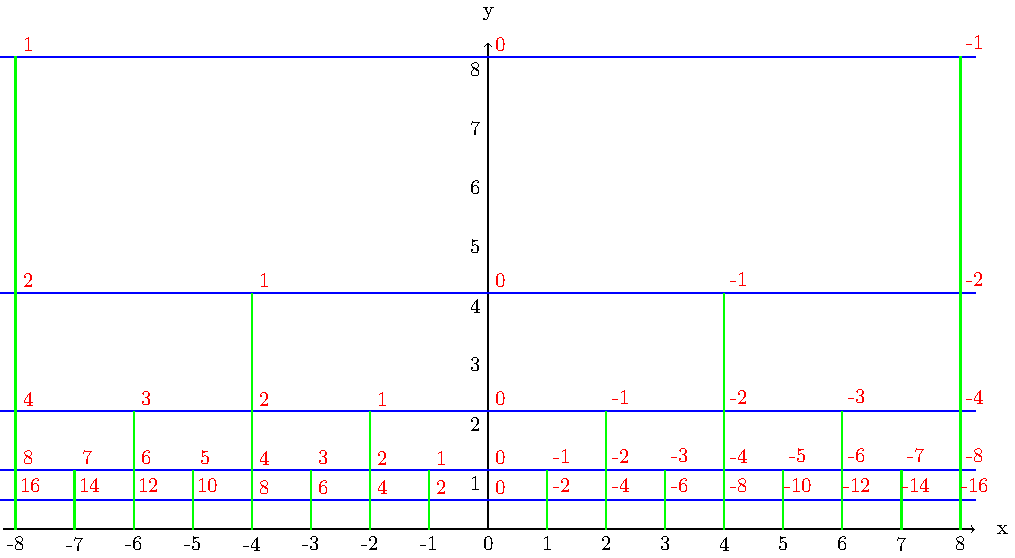
\includegraphics{images/01-grid-example-1}}
\caption{Rectilinear grid structure in \( \mathfrak{E}_1(1, \ln 2) \). Horizontal blue lines represent \(+1\) operations, vertical green lines represent \(\times 2\) operations. The red values are the assignment \(a = -x/y\).}
\label{fig:grid1_cs}
\end{figure}

\subsection{Arithmetic Torsion and the Local Area Law}

The non-commutativity of addition and multiplication gives rise to \textbf{arithmetic torsion}. For a single commutator step, \( (x \oplus_\mu \otimes_\lambda) - (x \otimes_\lambda \oplus_\mu) \), the torsion is \( \mu(1 - e^\lambda) \). When composed, this accumulates. In the \( \mathfrak{E}_1(1, \ln 2) \) grid, we observe a remarkable correspondence: the accumulated torsion between two different paths (e.g., multiply-then-add vs. add-then-multiply) is directly proportional to the hyperbolic area (number of grid cells) enclosed by those paths (Figure~\ref{fig:area-formula_cs}).

\begin{figure}[ht]
    \centering
    \resizebox{0.8\textwidth}{!}{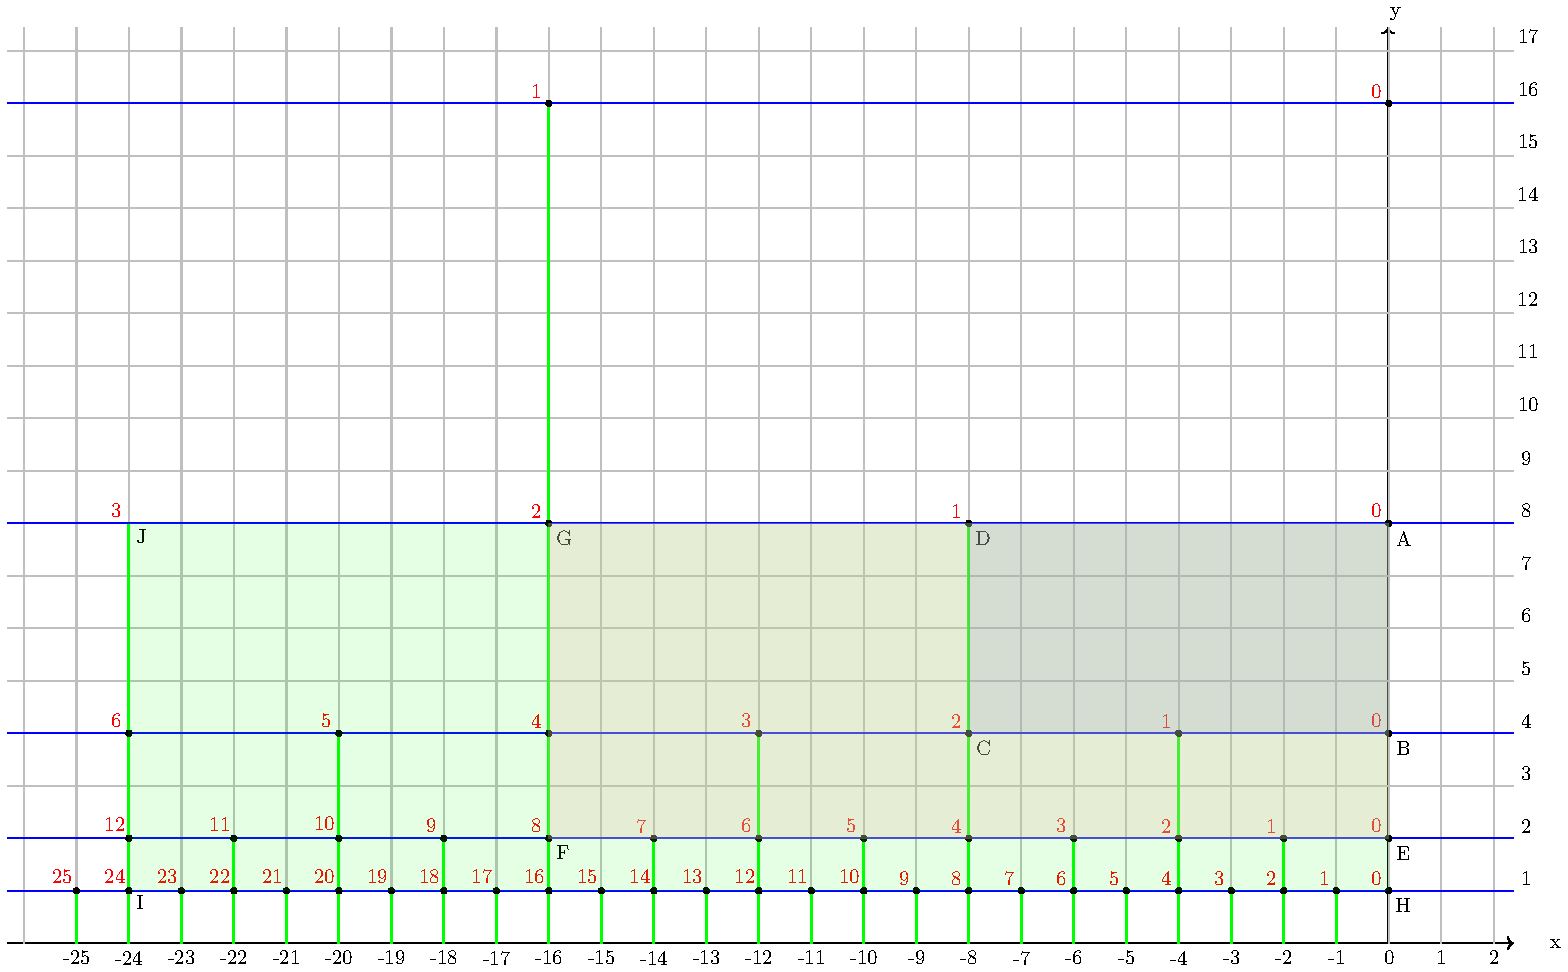
\includegraphics{images/17-area-formula}}
    \caption{Illustration of the correspondence between accumulated arithmetic torsion and the hyperbolic area enclosed by evaluation paths in \( \mathfrak{E}_1(1, \ln 2) \).}
    \label{fig:area-formula_cs}
\end{figure}

This macroscopic observation is underpinned by the microscopic law derived from the flow equation:
\begin{equation}
    d\tau = \mu \lambda\, du\, dv \label{eq:area_formula_diff_cs}
\end{equation}
where \( d\tau \) is the infinitesimal torsion generated by commuting infinitesimal additive (\(du\)) and multiplicative (\(dv\)) steps. This establishes that local arithmetic torsion acts as a geometric area density, suggesting it can be interpreted as a form of "arithmetic curvature".

\section{Global Torsion and the Accumulative Commutative Space}\label{sec:global_torsion_cs}

While Section~\ref{sec:propagation_grids_cs} established a local correspondence between torsion and area in the specific context of \( \mathfrak{E}_1 \), we now develop a general, global theory of arithmetic torsion applicable to any arbitrary arithmetic path. This requires introducing a new geometric stage: the Accumulative Commutative Space.

\subsection{Global Torsion and the Accumulative Commutative Space (ACS)}

The non-commutative nature of arithmetic operations means that evaluating a path \( \gamma \) and its reversed-sequence counterpart \( \bar{\gamma} \) yields different results. This "gap" or "tear" prevents the direct application of standard integral theorems. To quantify the total accumulated torsion, we need a space where paths can form closed boundaries.

We define the \textbf{global arithmetic torsion} \( \tau(\gamma) \) algebraically as the difference in evaluation between a path and its reverse:
\begin{equation}
\tau_{\text{alg}}(\gamma) = \nu(\gamma) - \nu(\bar{\gamma})
\label{eq:T_alg_formal_cs}
\end{equation}
This quantity is independent of the initial value, making it an intrinsic property of the path's operational structure.

To give this algebraic quantity a geometric meaning, we introduce the \textbf{Accumulative Commutative Space (ACS)}. This is a Euclidean plane whose coordinates are the commutative sums of the operational parameters along a path \( \gamma \):
\begin{itemize}
    \item \( A_\gamma = \sum \mu_k \): The total accumulated additive charge.
    \item \( M_\gamma = \sum \lambda_k \): The total accumulated logarithmic multiplicative charge.
\end{itemize}
In the ACS, any path \( \gamma \) and its reverse \( \bar{\gamma} \) share the same start point (0,0) and the same end point \( (A_\gamma, M_\gamma) \). Their trajectories, however, generally differ, thus enclosing a well-defined planar region \( \Sigma_\gamma \).

\subsection{The Triple Identity: A Stokes-like Theorem for Arithmetic}

Our central finding is that global arithmetic torsion possesses three equivalent formulations, bridging its algebraic definition with geometric measures in the ACS.

\begin{theorem}[The Triple Identity of Global Torsion]\label{thm:triple_identity_cs}
For an arbitrary arithmetic path \( \gamma \), its global torsion \( \tau(\gamma) \) is given by:
\begin{enumerate}
    \item \textbf{Algebraic Form:} \( \tau(\gamma) = \nu(\gamma) - \nu(\bar{\gamma}) \)
    \item \textbf{Interior Integral Form:} \( \tau(\gamma) = \iint_{\Sigma_\gamma} e^M dM \wedge dA \)
    \item \textbf{Boundary Integral Form:} \( \tau(\gamma) = \oint_{\partial \Sigma_\gamma} e^M dA \)
\end{enumerate}
where the integrals are taken over the region \( \Sigma_\gamma \) and its boundary \( \partial\Sigma_\gamma \) in the Accumulative Commutative Space.
\end{equation}

This triple identity provides a definitive answer to the "torsion-area problem": global arithmetic torsion is precisely quantified as an \( e^M \)-weighted area in the ACS. This establishes a concrete "Stokes-like theorem for arithmetic", relating a global algebraic effect to the integral of a local geometric density in a specially constructed parameter space. The ACS itself is not just a convenient tool; it also arises naturally as the target space for group homomorphisms from the free group of operations \( F_2 = \langle \oplus, \otimes \rangle \), giving it deep algebraic significance.

\section{The Tube Structure \( \mathcal{T} \) and Expression Dynamics}\label{sec:tube_structure_cs}

We now extend our view from a single geometric space to a \emph{family} of spaces to study how structures vary as the underlying operational strengths change. This leads to the concept of the "tube structure" \( \mathcal{T} \).

\subsection{Family of Expression Spaces Indexed by \( \lambda \)}

Let us fix \( \mu=1 \) and consider the family of spaces \( \{ \mathfrak{E}_1^{(\lambda)} \}_{\lambda \in \Lambda} \) generated by varying the multiplicative parameter \( \lambda \). Each space \( \mathfrak{E}_1^{(\lambda)} \) is a "slice" in this family.

\begin{definition}[Tube Structure \( \mathcal{T} \)]\label{def:tube_structure_cs}
The \textbf{tube structure} \( \mathcal{T} \) is the total space formed by the family of slices \( \{ \mathfrak{E}_1^{(\lambda)} \}_{\lambda \in \Lambda} \). It can be written as the disjoint union \( \mathcal{T} = \bigsqcup_{\lambda \in \Lambda} \mathfrak{E}_1^{(\lambda)} \), equipped with a structure (e.g., a fiber bundle) that relates the different fibers. \( \Lambda \) is the base space and \( \mathfrak{E}_1^{(\lambda)} \) is the fiber over \( \lambda \).
\end{definition}

\subsection{Sections, Trajectories, and Zero Loci in \( \mathcal{T}_1 \)}

Within \( \mathcal{T} \), we can track how arithmetic constructs evolve with \( \lambda \). A fixed algebraic structure (like a polynomial) traces a path, called a \textbf{section}, through the tube as \( \lambda \) varies.

A key feature to analyze is the **zero locus**: the set of points where the assignment function is zero. In the tube \( \mathcal{T}_1 \) built from \( \mathfrak{E}_1^{(\lambda)} \) spaces, the zero locus in every slice is the y-axis (\( x=0 \)), as \( a = -x/y \). This locus is constant and does not evolve with \( \lambda \).

\subsection{Outlook: Nontrivial Tube Spaces and Topological Change}

The simplicity of the zero locus in \( \mathcal{T}_1 \) limits its ability to model more complex phenomena. This motivates the search for \textbf{"non-trivial" arithmetic expression spaces}, \( \mathfrak{E}_{NT} \), where the assignment function or geometry might allow for more complex zero sets within each slice (e.g., multiple curves).

In a tube structure \( \mathcal{T}_{NT} \) built from such spaces, the zero locus could exhibit rich, dynamic behavior as \( \lambda \) varies, including morphing, bifurcation, and topological change. Analyzing these phenomena is a crucial direction for future research, potentially connecting AEG to algebraic geometry, dynamical systems, and knot theory.

\section{Discussion and Future Directions}\label{sec:discussion_future}

This paper has laid the initial groundwork for Arithmetic Expression Geometry. We have moved from algebraic paths to a governing flow equation, a concrete hyperbolic realization (\( \mathfrak{E}_1 \)), and a global theory of torsion. This concluding section synthesizes these findings and outlines key avenues for future research.

\subsection{Levels of Equality and Foundational Problems}

From a foundational perspective, different levels of equality can be considered:
\begin{enumerate}
    \item \textbf{Literal Equality:} Identical sequences of operations.
    \item \textbf{Operational/Syntactic Equality:} Equality under rules like associativity.
    \item \textbf{Relational/Algebraic Equality:} Equality under additional imposed relations (e.g., from group theory).
    \item \textbf{Semantic Equality:} Equality of the final numerical evaluation.
\end{enumerate}
The "distance" between these levels gives rise to significant challenges. For instance, a syntactically valid expression (e.g., \( 1 \div (x-x) \)) may not be semantically valid. How do such singularities manifest in the geometric model? Do they correspond to geometric singularities in the space? What is the relationship between algebraic symmetries (e.g., automorphisms of the generating group) and geometric symmetries (e.g., isometries of the space)? Exploring these questions is central to developing a complete theory.

\subsection{Future Research Directions}

This foundational work opens numerous avenues for further research:

\begin{enumerate}[label=\textbf{F\arabic*.}, leftmargin=*, widest=F6, align=left]
    \item \textbf{A General Arithmetic Gauss-Bonnet Theorem:} A primary goal is to fully bridge the local and global pictures of torsion. This involves relating the integral of the torsion density (or a related curvature) in a space like \( \mathfrak{E}_1 \) to the global algebraic torsion, potentially yielding a Gauss-Bonnet type theorem for AEG.

    \item \textbf{Construction and Analysis of Non-Trivial Spaces (\( \mathfrak{E}_{NT} \)):} A crucial next step is to construct and investigate "non-trivial" AEG spaces (\( \mathfrak{E}_{NT} \)) that exhibit more complex zero-set behavior, allowing for the study of bifurcation and topological change within their tube structures.

    \item \textbf{Connections to Other Mathematical Fields:}
        \begin{itemize}
            \item \textit{Geometric Group Theory:} Deepen the connection between AEG grid structures and the geometry of Cayley graphs for groups like BS(m,n) and other solvable or hyperbolic groups.
            \item \textit{Knot Theory and Topology:} Explore whether the evolution of zero loci in tube structures can model knot invariants like the Alexander polynomial, which arise from related algebraic structures.
            \item \textit{Number Theory:} Investigate potential AEG constructions related to number-theoretic functions, continued fractions, or modular groups.
        \end{itemize}

    \item \textbf{Global Metric Existence:} Resolve the open problem of finding conditions under which a global metric exists on a manifold \( S \) that makes a given function \( a: S \to \mathbb{R} \) satisfy the Arithmetic Flow Equation globally.
\end{enumerate}

\subsection{Concluding Remark}

Arithmetic Expression Geometry offers a nascent but potentially unifying perspective, weaving together threads from computation, algebra, and geometry. By treating arithmetic evaluation as a dynamic geometric process, AEG reveals unexpected structures and provides quantitative links between algebraic properties and geometric measures. The rich set of open problems suggests that further exploration of this geometry holds significant promise for uncovering deeper connections between the way we compute and the mathematical spaces that computation might naturally inhabit.

\newpage
\appendix

\section{Formal Solution of the Arithmetic Flow Equation}\label{app:flow_solution}

This appendix provides the derivation of the formal solution to the Arithmetic Flow Equation~\eqref{eq:flow_cs}, \( \frac{da}{ds} = \mu \cos \theta + a \lambda \sin \theta \), assuming constant parameters. This is a first-order linear ODE. Rewriting in standard form \( \frac{da}{ds} - (\lambda \sin \theta) a = \mu \cos \theta \), we use the integrating factor \( I(s) = e^{-\lambda s \sin \theta} \).
Multiplying by \( I(s) \) gives:
\[
\frac{d}{ds}\left( a e^{-\lambda s \sin \theta} \right) = \mu \cos \theta e^{-\lambda s \sin \theta}
\]
Integrating both sides with respect to \( s \) (for \( \sin \theta \neq 0 \)):
\[
a e^{-\lambda s \sin \theta} = \mu \cos \theta \left( \frac{e^{-\lambda s \sin \theta}}{-\lambda \sin \theta} \right) + C_1
\]
Solving for \( a(s) \) gives \( a(s) = -\frac{\mu}{\lambda} \cot \theta + C_1 e^{\lambda s \sin \theta} \). Applying the initial condition \( a(0) = a_0 \) determines the constant \( C_1 = a_0 + \frac{\mu}{\lambda} \cot \theta \). Substituting back gives the final solution:
\begin{equation}
   a(s) = \left(a_0 + \frac{\mu}{\lambda} \cot \theta\right) e^{\lambda s \sin \theta} - \frac{\mu}{\lambda} \cot \theta \quad (\text{for } \sin \theta \neq 0) \label{eq:solution_appendix_cs}
\end{equation}

\section{Geometric Calculation Details for \( \mathfrak{E}_1 \)}\label{app:geometry_calc}

\subsection{Proof of Theorem~\ref{thm:generalE1_cs}}
The differential of the assignment is \( da = d(-x/y) = (x dy - y dx) / y^2 = -(dx + a dy) / y \).
The arc length differential is \( ds = \frac{1}{y} \sqrt{dx^2/\mu^2 + dy^2/\lambda^2} \).
The directional derivative is \( \frac{da}{ds} = -\frac{dx + a dy}{\sqrt{dx^2/\mu^2 + dy^2/\lambda^2}} \).
We can rewrite the numerator as \( -dx - a dy = \mu(-dx/\mu) + a\lambda(-dy/\lambda) \).
Define the direction angle \( \theta \) via its cosines:
\[
\cos \theta = \frac{-dx/\mu}{\sqrt{dx^2/\mu^2 + dy^2/\lambda^2}} \quad \text{and} \quad \sin \theta = \frac{-dy/\lambda}{\sqrt{dx^2/\mu^2 + dy^2/\lambda^2}}
\]
Substituting these into the expression for \( da/ds \) gives:
\[
\frac{da}{ds} = \frac{\mu(-dx/\mu) + a\lambda(-dy/\lambda)}{\sqrt{dx^2/\mu^2 + dy^2/\lambda^2}} = \mu \cos \theta + a \lambda \sin \theta
\]
This completes the proof.

\subsection{Infinitesimal Arithmetic Torsion}
We derive \( d\tau = \mu \lambda \, du \, dv \). Consider applying infinitesimal steps: \( du \) in the \( \mu \)-direction and \( dv \) in the \( \lambda \)-direction, from value \( a \).
\begin{itemize}
    \item Path 1: \( (a + \mu du) e^{\lambda dv} \)
    \item Path 2: \( a e^{\lambda dv} + \mu du \)
\end{itemize}
The torsion \( d\tau \) is the difference. Using \( e^x \approx 1+x \):
\begin{align*}
d\tau &\approx (a + \mu du) (1 + \lambda dv) - (a (1 + \lambda dv) + \mu du) \\
&= (a + a \lambda dv + \mu du + \mu \lambda du dv) - (a + a \lambda dv + \mu du) = \mu \lambda du dv
\end{align*}

% --- Bibliography Commands ---
\bibliographystyle{plain}
\bibliography{aeg-paper} % Your .bib file name

\end{document}
